\chapter{Tinjauan Pustaka dan Dasar Teori}

\section{Tinjauan Pustaka}

Pengujian mengenai pengaruh jumlah \textit{hidden layer} terhadap kinerja jaringan saraf tiruan (JST) telah banyak dilakukan oleh berbagai peneliti. Perbedaan jumlah 
\textit{hidden layer} terbukti memengaruhi kemampuan jaringan dalam melakukan klasifikasi, kecepatan pelatihan, serta kemampuan generalisasi terhadap data baru. 
Beberapa hasil penelitian yang relevan disajikan berikut ini.

Surkan dan Singleton (1995) \cite{NeuralNetforBondRating} dalam penelitiannya membuat sebuah JST berdasarkan rating obligasi dari moody’s or standard and poor’s. 
Data yang digunakan berisi tujuh buah \textit{feature} dan 126 \textit{instance} pola obligasi. Moody’s memisahkan rating obligasi menjadi tujuh kelas, yaitu Aaa, Aal, Aa2, Aa3, A1 , A2, dan A3. Aaa 
dikategorikan sebagai kualitas tinggi, Aa1-Aa3 sebagai kualitas menengah, dan A1-A3 sebagai kualitas rendah. Jaringan syaraf tiruan yang dibuat akan digunakan untuk 
membedakan kelas kualitas tinggi (Aaa) dan kelas kualitas rendah (A1-A3). JST dibuat dengan tiga model arsitektur. satu dari tiga model menggunakan satu \textit{hidden layer}. 
Dua model lainnya menggunakan dua \textit{hidden layer} dengan jumlah \textit{neuron} yang berbeda, yaitu masing - masing memiliki arsitektur
[7-14-2], [7-5-10-2], dan [7-10-5-2]. Hasilnya menunjukkan bahwa arsitektur dengan dua \textit{hidden layer} memberikan akurasi yang lebih tinggi. Arsitektur [7-10-5-2] mencapai 
akurasi 88\% pada data uji, sedangkan [7-14-2] yang hanya mencapai 65\%. Penelitian ini menyimpulkan bahwa penggunaan dua \textit{hidden layer} dapat meningkatkan 
kinerja klasifikasi tanpa secara signifikan memperlama waktu pelatihan.

De Villiers dan Barnard (1993) \cite{backpropagationwith1and2} mengevaluasi perbedaan kinerja antara jaringan 
saraf tiruan (JST) satu \textit{hidden layer} dengan dua \textit{hidden layer}. Studi ini menggunakan pendekatan “\textit{distribution of distributions}”. 
Metode tersebut menggunakan sejumlah dataset acak dari beragam distribusi \textit{Gaussian} untuk mensimulasikan variasi alami pada data pelatihan.
Dalam setiap eksperimen, kompleksitas jaringan dikendalikan agar tetap konstan dengan menyamakan jumlah total bobot antar arsitektur 
(± 20, 40, atau 60 bobot). Dengan cara ini, perbandingan kinerja berfokus pada pengaruh kedalaman topologi, bukan pada perbedaan kapasitas model.
Hasil penelitian menunjukkan bahwa, secara rata-rata, jaringan satu \textit{hidden layer} menghasilkan kinerja pelatihan (training) dan 
generalisasi yang lebih stabil dibandingkan jaringan dua \textit{hidden layer}, yang cenderung lebih sensitif terhadap inisialisasi bobot dan 
lebih sering terjebak pada local minima. Namun, beberapa konfigurasi jaringan dua \textit{hidden layer} khususnya ketika jumlah neuron pada dua 
\textit{hidden layer} relatif seimbang menunjukkan konvergensi yang lebih cepat dan kadang mencapai performa setara dengan jaringan satu \textit{hidden layer}.
Penelitian ini juga menegaskan bahwa peningkatan jumlah sampel pelatihan secara signifikan meningkatkan akurasi klasifikasi pada 
kedua arsitektur, serta memperkecil variabilitas hasil antar pelatihan. Secara keseluruhan, temuan tersebut menunjukkan bahwa 
penambahan \textit{hidden layer} tidak otomatis meningkatkan performa bila kompleksitas jaringan dan jumlah data tetap terbatas, meskipun 
dapat memberikan keuntungan efisiensi pelatihan pada kondisi topologi tertentu.

Berdasarkan penelitian Panchal (2011) \cite{Panchal2011}, metode \textit{Hopfield Neural Networks} dan \textit{Akaike’s Information Criterion} (AIC) digunakan untuk menentukan 
jumlah \textit{hidden layer} dan jumlah \textit{neuron} yang optimal. Pendekatan ini digunakan untuk menghindari masalah 
\textit{overfitting} dan \textit{underfitting} dengan memilih arsitektur jaringan yang sesuai dengan kompleksitas data. Hasil eksperimen menunjukkan 
bahwa penambahan jumlah \textit{hidden layer} secara signifikan meningkatkan \textit{Correct Classification Rate} (CCR) dan menurunkan \textit{error}, meskipun diiringi dengan peningkatan waktu pelatihan. 
Hasil penelitiannya menyimpulkan bahwa dalam aplikasi yang 
memprioritaskan akurasi tinggi, penambahan \textit{hidden layer} dapat memberikan peningkatan performa yang signifikan. 
Sebaliknya, untuk aplikasi yang memerlukan waktu respons cepat atau sumber daya komputasi terbatas, penggunaan satu \textit{hidden layer} 
sudah dianggap cukup memadai. Dengan demikian, pemilihan arsitektur dapat disesuaikan secara fleksibel berdasarkan 
\textit{trade-off} antara akurasi dan efisiensi komputasi.

Thomas (2017) \cite{Thomas2017} melakukan studi untuk menguji perbandingan antara jaringan dengan satu \textit{hidden layer} 
(\textit{Single Hidden Layer Feedforward Network}, SLFN) dan dua \textit{hidden layer} (\textit{Two-Layer Feedforward Network}, TLFN). Penelitian ini menggunakan sepuluh 
dataset publik dari berbagai domain (seperti \textit{Abalone, Airfoil Noise, Concrete}, dan \textit{White Wine Quality}) serta algoritma pelatihan Levenberg–Marquardt. 
Hasil eksperimen menunjukkan bahwa sembilan dari sepuluh dataset menghasilkan \textit{error} yang lebih rendah pada arsitektur dengan dua \textit{hidden layer}. Secara rata-rata, 
jaringan dengan dua \textit{hidden layer} menunjukkan peningkatan performa sebesar 5–6\% dibandingkan jaringan dengan satu \textit{hidden layer}. Penelitian ini menyimpulkan bahwa 
dua \textit{hidden layer} umumnya memberikan kemampuan generalisasi yang lebih baik, khususnya pada dataset kompleks, meskipun peningkatan tersebut bergantung pada 
karakteristik data dan tingkat \textit{noise} yang ada.

Artikel dari Uzair dan Jamil (2020) \cite{Uzair} mengkaji berbagai hasil penelitian mengenai pengaruh jumlah \textit{hidden layer} terhadap kompleksitas waktu dan 
akurasi dalam jaringan saraf tiruan. Hasil kajian menunjukkan bahwa menentukan jumlah \textit{hidden layer} yang optimal tidak dapat 
hanya didasarkan pada jumlah \textit{input layer} dan \textit{output} saja. Meskipun terdapat berbagai metode untuk memperkirakannya, akurasi 
aproksimasi sangat bergantung pada karakteristik data yang digunakan. Apabila tujuannya adalah mencapai akurasi tinggi, arsitektur 
jaringan yang lebih dalam dapat menjadi pilihan. Namun, jika efisiensi waktu menjadi prioritas, penggunaan jaringan yang dalam 
kurang tepat digunakan. Selain itu, penambahan \textit{neuron} atau \textit{hidden layer} yang berlebihan berisiko menyebabkan \textit{overfitting}. Oleh 
karena itu, sangat disarankan untuk melakukan analisis awal terhadap sampel data guna memperkirakan konfigurasi \textit{hidden layer} yang sesuai.

Dari berbagai penelitian di atas, dapat disimpulkan bahwa penambahan jumlah \textit{hidden layer} umumnya dapat meningkatkan kemampuan jaringan dalam mengenali pola 
yang kompleks, tetapi tidak selalu memberikan peningkatan signifikan jika jumlah data atau kompleksitas model terbatas. Semakin banyak \textit{hidden layer} 
akan meningkatkan waktu pelatihan dan risiko \textit{overfitting}. Oleh karena itu, pemilihan jumlah \textit{hidden layer} yang optimal harus mempertimbangkan 
keseimbangan antara akurasi, generalisasi, dan efisiensi komputasi.

Pada penelitian ini, penulis akan membangun jaringan saraf tiruan dengan jumlah \textit{hidden layer} dan \textit{neuron} yang bervariasi, untuk kemudian dibandingkan 
berdasarkan akurasi dan waktu komputasi yang dihasilkan. Data yang digunakan merupakan data dimensi tinggi dan lebar suatu barang. Data akan diklasifikasikan menjadi 
tiga kategori, yaitu wardrobe, lemari, dan buffet. Melalui penelitian ini diharapkan dapat diperoleh pemahaman yang lebih jelas mengenai pengaruh jumlah \textit{hidden layer} 
terhadap kinerja jaringan saraf tiruan dalam konteks klasifikasi berbasis dimensi objek.

\begin{table}[H]
\centering
\caption{Ringkasan Penelitian Terdahulu Mengenai Jumlah Hidden Layer pada Jaringan Saraf Tiruan}
\label{tab:tinjauan-hiddenlayer}
\renewcommand{\arraystretch}{1.3}
\setlength{\tabcolsep}{3pt}
\begin{tabular}{|c|p{2cm}|p{3cm}|p{2cm}|p{2cm}|p{4cm}|}
\hline
\textbf{No} & \textbf{Peneliti (Tahun)} & \textbf{Judul / Konteks Penelitian} & \textbf{Jumlah Hidden Layer yang Diuji} & \textbf{Dataset / Aplikasi} & \textbf{Kesimpulan} \\
\hline

1 & Surkan \& Singleton (1995) &
\textit{Neural Networks for Bond Rating Improved by Multiple Hidden Layers} &
1 HL: [7–14–2]; 2 HL: [7–5–10–2], [7–10–5–2] &
126 data obligasi (Moody’s \& S\&P) &
Dua \textit{hidden layer} meningkatkan akurasi klasifikasi tanpa memperlama waktu pelatihan secara signifikan. \\
\hline

2 & De Villiers \& Barnard (1993) &
\textit{Backpropagation Neural Nets with One and Two Hidden Layers} &
1 HL dan 2 HL (20–60 bobot total) &
Dataset sintetis Gaussian dan data nyata &
Penambahan \textit{hidden layer} tidak selalu meningkatkan kinerja; tergantung pada kompleksitas data dan topologi jaringan. \\
\hline

\end{tabular}
\end{table}

\begin{table}[H]
\centering\renewcommand{\arraystretch}{1.3}
\setlength{\tabcolsep}{3pt}
\begin{tabular}{|c|p{2cm}|p{3cm}|p{2cm}|p{2cm}|p{4cm}|}
\hline
\textbf{No} & \textbf{Peneliti (Tahun)} & \textbf{Judul / Konteks Penelitian} & \textbf{Jumlah Hidden Layer yang Diuji} & \textbf{Dataset / Aplikasi} & \textbf{Kesimpulan} \\
\hline

3 & Panchal et al. (2011) &
\textit{Behaviour Analysis of MLPs with Multiple Hidden Neurons and Hidden Layers} &
1–4 HL, variasi jumlah \textit{neuron} &
Data retensi karyawan (9–17 \textit{feature}) &
1 HL cukup untuk masalah sederhana, 2 HL cocok untuk pola kompleks; AIC efektif untuk menentukan arsitektur optimal. \\
\hline

4 & Thomas et al. (2017) &
\textit{Two Hidden Layers Are Usually Better Than One} &
1 HL (SLFN) vs 2 HL (TLFN) &
10 dataset publik (UCI, MATLAB, Bilkent, dll.) &
Dua \textit{hidden layer} umumnya memberikan generalisasi lebih baik, terutama untuk dataset kompleks. \\
\hline

5 & Uzair \& Jamil (2020) &
\textit{Effects of Hidden Layers on the Efficiency of Neural Networks} &
1–5 HL (studi literatur dan analisis empiris) &
Kajian berbagai penelitian terdahulu &
Tiga \textit{hidden layer} memberikan keseimbangan terbaik antara akurasi dan efisiensi waktu; lebih banyak \textit{layer} meningkatkan risiko \textit{overfitting}. \\
\hline
\end{tabular}
\end{table}


\section{Dasar Teori}

\subsection{Persamaan linear diskriminan}

Diskriminan merupakan sebuah fungsi yang menerima vektor input ${x} \quad \mathbf{x}$ dan mengelompokkannya ke dalam K kelas. Kelas tersebut disimbolkan sebagai $C_k$,
dengan $k = 1, 2, 3,...,K$. Kelas-kelas ini akan dipisahkan oleh satu atau lebih \textit{decision boundary} yang berupa \textit{hyperplane} \cite{bishop_2006}. 
Tujuan dari proses klasifikasi adalah untuk menetapkan setiap masukan tepat ke kelas-nya masing-masing. Persamaan linear diskriminan dituliskan sebagai berikut:
\begin{equation}
    y(\textbf{x}) = \textbf{w}^T \textbf{x} + w_0
    \label{eq:wx+b}
\end{equation}
% Atau dalam vektor dapat ditulis:
% \begin{equation}
%     y(\textbf{x}) = \textbf{w}^T \textbf{x} + w_0
%     \label{eq:wx+b Vektor}
% \end{equation}

Dalam persamaan tersebut, $\textbf{w}$ disebut sebagai vektor bobot, sedangkan $\textbf{w}^T$ menyatakan \textit{transpose} dari vektor bobot. 
Sementara itu, $w_0$ disebut juga sebagai bias dan dapat dilambangkan dengan variabel $b$. 
Pada permasalahan klasifikasi biner sebuah masukan $\textbf{x}$ diklasifikasikan ke dalam kelas $C_1$ jika $y(\textbf{x}) \geq 0$. 
Namun, jika $y(\textbf{x}) \leq 0$ maka $\textbf{x}$ dikategorikan ke dalam kelas $C_2$.
Kedua kelas ini akan dipisahkan oleh sebuah \textit{decision boundary}. 
\textit{Decision boundary} sendiri didefinisikan oleh persamaan $y(\textbf{x}) = 0$. \textit{Decision boundary} akan merepresentasikan sebuah \textit{hyperplane} berdimensi (D - 1) pada masukan berdimensi D. 
Sebagai contoh apabila masukan memiliki 2 \textit{feature} (D = 2), maka data tersebut dapat direpresentasikan oleh bidang kartesius dengan dua sumbu. 
Pada kondisi ini, \textit{decision boundary} akan berdimensi satu dan berbentuk garis yang memisahkan kedua kelas pada \textit{input space}. 
\textit{Decision boundary} ini berkaitan erat dengan vektor bobot $\textbf{w}$ dan bias $w_0$. 
Sebagai ilustrasi, misalkan terdapat dua titik $\textbf{x}_A$ dan $\textbf{x}_B$ yang keduanya berada pada \textit{decision boundary} sehingga $y(\textbf{x}_A) = y(\textbf{x}_B) = 0$. Dengan demikian berlaku hubungan berikut:
\begin{equation}
    \textbf{w}^T(\textbf{x}_A - \textbf{x}_B) = 0
\end{equation}

Persamaan tersebut menunjukan bahwa vektor bobot $\textbf{w}$ tegak lurus terhadap setiap vektor yang terletak pada \textit{decision boundary}\cite{bishop_2006}. 
Oleh karena itu, vektor $\textbf{w}$ menentukan orientasi dari \textit{decision boundary}. 
Apabila $\textbf{x}$ berada pada \textit{decision boundary}, maka $y(\textbf{x})=0$. Jarak normal dari titik \((0,0)\) ke \textit{decision boundary} dapat dituliskan sebagai berikut :
\begin{equation}
    \frac{\textbf{w}^T \textbf{x}}{||\textbf{w}||} = -\frac{w_0}{||\textbf{w}||}
    \label{eq: jarak origin ke decision boundary}
\end{equation}

Dapat dilihat bahwa $w_0$ akan menentukan posisi dari \textit{decision boundary}. Sebagai contoh diberikan  data masukan dan keluaran dari fungsi OR seperti pada tabel \ref{tab : Dataset OR}.
\begin{table}[!ht]
    \caption{Masukan dan Keluaran fungsi OR}
    \centering
    \begin{tabular}{||l|l|l|l||}
    \hline
        $x_0$ & $x_1$ & output & y  \\ [0.5ex]
        \hline\hline
        0 & 0 & 0 & -1  \\ \hline
        0 & 1 & 1 & 1  \\ \hline
        1 & 0 & 1 & 1  \\ \hline
        1 & 1 & 1 & 1  \\ \hline
    \end{tabular}
    \label{tab : Dataset OR}
\end{table}

Pada data tersebut berisi empat buah \textit{instance} dan memiliki 2 buah \textit{feature}. Karena memiliki 2 buah \textit{feature} maka masukan berdimensi 2 atau D = 2. Masukan akan dibedakan menjadi 2 kelas yaitu $C_1$ untuk $y \geq 0$ dan kelas $C_2$ untuk $y \leq 0$. Untuk memisahkan kedua kelas tersebut akan dipilih nilai $\textbf{w}$ dan $w_0$. \textit{Decision boundary} yang dibentuk akan memiliki satu dimensi.

\begin{figure}[htbp]
    \centering
    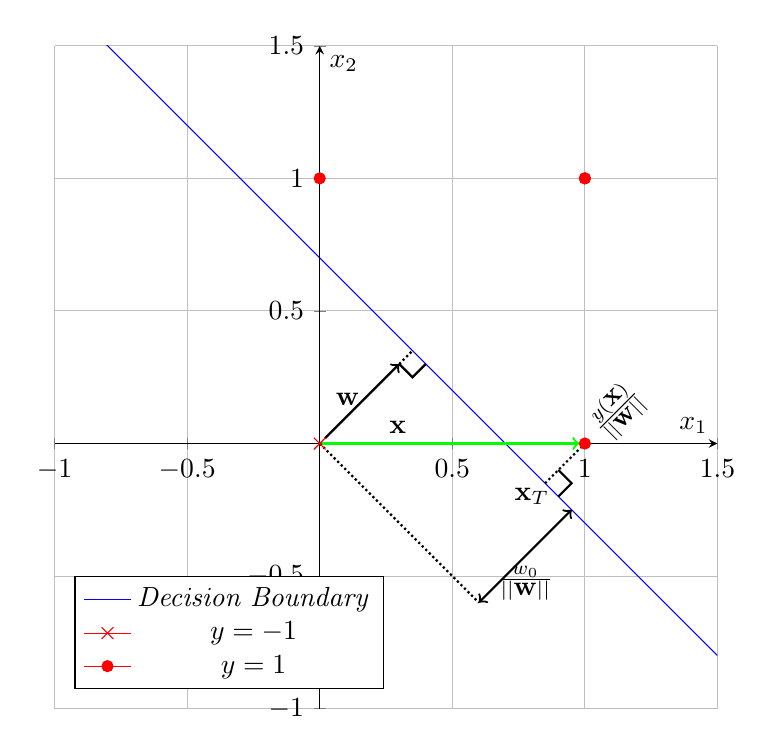
\begin{tikzpicture}
        \begin{axis}[
            xlabel=$x_1$,
            ylabel=$x_2$,
            xmin=-1, xmax=1.5,
            ymin=-1, ymax=1.5,
            grid=major,
            width=10cm,
            height=10cm,
            domain=-2:4,
            samples=100,
            legend pos=south west,
            axis lines=middle, % Add this line to get the axes in the middle
        ]
        \addplot[color=blue]{-x+0.7};
        % Adding x and y axis
        \draw [dashed] (axis cs:0,-6) -- (axis cs:0,6) node [above] {$x=0$};
        \draw [dashed] (axis cs:-2,0) -- (axis cs:4,0) node [right] {$y=0$};

        % Adding points
        \addplot[mark=x, color=red, mark size = 3] coordinates {(0,0)};
        \addplot[mark=*, color=red, mark size = 2] coordinates {(0,1)};
        \legend{\textit{Decision Boundary}, $y = -1$, $y = 1$}
        \addplot[mark=*, color=red, mark size = 2] coordinates {(1,0)};
        \addplot[mark=*, color=red, mark size = 2] coordinates {(1,1)};
        \addplot[mark=*, color=red, mark size = 2] coordinates {(1,1)};

        % Adding vector
        \draw[->, thick] (axis cs:0.02,0.02) -- (axis cs:0.3,0.3) node[pos=0.3, above] {$\textbf{w}$};
        \draw[->, thick, color=green] (axis cs:0,0) -- (axis cs:0.98,0) node[pos=0.3, above, color=black] {$\textbf{x}$};
        \draw[thick, densely dotted] (axis cs:0.3,0.3) -- (axis cs:0.35,0.35);
        \draw[<->, thick] (axis cs:0.6,-0.6) -- (axis cs:0.95,-0.25) node[midway, below] {$\frac{w_0}{||\textbf{w}||}$};
        \draw[densely dotted, thick] (axis cs:0.85,-0.15) -- (axis cs:1,0) node[pos=1, right, rotate=45, xshift =1mm] {$\frac{y(\textbf{x})}{||\textbf{w}||}$};
        \node at (axis cs:0.8,-0.2) {$\textbf{x}_T$};
        \draw[densely dotted, thick] (axis cs:0,0) -- (axis cs:0.6,-0.6);
        \draw[-, thick] (axis cs:0.3,0.3) -- (axis cs:0.35,0.25) -- (axis cs:0.4,0.3);
        \draw[-, thick] (axis cs:0.9,-0.1) -- (axis cs:0.95,-0.15) -- (axis cs:0.9,-0.2);
        \end{axis}
    \end{tikzpicture}
    \caption{Ilustrasi bagaimana fungsi OR dapat dipisahkan menjadi 2 kelas.}
    \label{fig:plot or}
\end{figure}

Dari Gambar \ref{fig:plot or} dapat dilihat bahwa terdapat \textit{decision boundary} yang memisahkan kedua kelas. 
Vektor $\textbf{w}$ tegak lurus dengan \textit{decision boundary}, dan jarak antara \textit{decision boundary} dan titik origin adalah $\frac{w_0}{||\textbf{w}||}$. 
Selanjutnya, untuk mengetahui jarak antara sebuah titik dengan \textit{decision boundary}, digunakan Persamaan \ref{eq: 2.5}.
\begin{equation}
    r = \frac{y(\textbf{x})}{||\textbf{w}||}
    \label{eq: 2.5}
\end{equation}
Hal ini dapat dibuktikan dengan memisalkan $\textbf{x}_T$ sebagai proyeksi dari titik $\textbf{x}$ pada \textit{decision boundary}. 
Dengan demikian, vektor $\textbf{x}$ dapat dituliskan seperti pada Persamaan \ref{eq: 2.6}.
\begin{equation}
    \textbf{x} = \textbf{x}_T + r \frac{\textbf{w}}{||\textbf{w}||}
    \label{eq: 2.6}
\end{equation}
Dengan mengalikan Persamaan \ref{eq: 2.6} dengan $\textbf{w}^T$ dan menambahkan $w_0$, diperoleh Persamaan \ref{eq: 2.7}.
\begin{equation}
    \textbf{w}^T \textbf{x} + w_0 = \textbf{w}^T \textbf{x}_T + w_0 + r \frac{\textbf{w}^T \textbf{w}}{||\textbf{w}||}
    \label{eq: 2.7}
\end{equation}
Dengan mensubtitusikan Persamaan \ref{eq:wx+b}, kondisi $\textbf{w}^T \textbf{x}_T + w_0 = 0$ untuk titik pada \textit{decision boundary}, serta identitas $\frac{\textbf{w}^T \textbf{w}}{||\textbf{w}||} = ||\textbf{w}||$ ke dalam Persamaan \ref{eq: 2.7}, diperoleh Persamaan \ref{eq: 2.5}. 

Setelah penjelasan mengenai hubungan antara vektor bobot dengan \textit{decision boundary}, sering kali dilakukan penyederhanaan notasi agar memudahkan manipulasi matriks.
Salah satu cara yang umum digunakan adalah menggabungkan bias ke dalam vektor bobot. 
Penggabungan ini tidak mengubah makna persamaan, tetapi memungkinkan seluruh operasi dituliskan dalam bentuk perkalian vektor. 
Hal ini dilakukan dengan menambahkan sebuah \textit{dummy input} $x_0 = 1$, lalu mendefinisikan $\hat{w} = (w_0, \textbf{w})$ dan $\hat{x} = (x_0, \textbf{x})$, 
sehingga fungsi dapat dituliskan kembali sebagai Persamaan \ref{eq: 2.8}.
\begin{equation}
    y(\textbf{x})=\hat{\textbf{w}}^T\hat{\textbf{x}}
    \label{eq: 2.8}
\end{equation}
\textit{Decision boundary} dalam sebuah model klasifikasi saling terikat melalui vektor bobot, sehingga penentuan bobot tersebut akan sangat memengaruhi hasil 
klasifikasi. Untuk mendapatkan bobot yang optimal, salah satu pendekatan yang umum digunakan adalah metode \textit{machine learning}. Dalam konteks ini, 
Jaringan Syaraf Tiruan menjadi salah satu teknik yang efektif karena mampu mempelajari pola dan hubungan kompleks antar \textit{feature} secara otomatis.

\subsection{Jaringan Syaraf Tiruan}
Jaringan Syaraf Tiruan (JST) merupakan salah satu metode dalam \textit{machine learning} yang digunakan untuk mempelajari pola dari data. 
\textit{Machine learning} sendiri adalah sebuah subset dari Kecerdasan Artifisial (KA) yang berfokus pada pengembangan algoritma yang dapat belajar dari data dan 
meningkatkan performanya seiring waktu tanpa harus diprogram secara eksplisit. 
Ketiga istilah tersebut memiliki bidang ilmu yang saling beririsan. Untuk memahami hubungan antara bidang ilmu tersebut, hubungan ketiganya dapat dilihat pada Gambar \ref{fig:diagram_venn}.

\begin{figure}[H]
    \centering
    \includegraphics[width = 7cm]{contents/chapter-2/diagram_venn.png}
    \caption{Diagram Venn ini menggambarkan hubungan antara bidang ilmu \cite{GoodBengCour16}}
    \label{fig:diagram_venn}
\end{figure}

Jaringan Syaraf Tiruan pada awalnya terinspirasi dari jaringan syaraf biologis pada otak manusia\cite{Kelleher2019-cj}. 
Pada otak manusia \textit{neuron-neuron} berkomunikasi satu sama lain melalui suatu sinyal listrik. 
Sinyal tersebut diteruskan dari satu \textit{neuron} ke \textit{neuron} lainnya melalui mekanisme yang dikenal sebagai \textit{action potensial}. 
Seperti pada Gambar \ref{fig:action potential}. \textit{Neuron-neuron} yang saling terhubung ini memiliki tingkat kekuatan koneksi tertentu atau \textit{synaptic strength}.

\begin{figure}[H]
    \centering
    \includegraphics[width=8cm]{contents/chapter-2/action potential.png}
    \caption{\textit{Action Potential} pada jaringan syaraf}
    \label{fig:action potential}
\end{figure}

\textit{Action Potential} (AP) adalah sinyal listrik yang bergerak sepanjang akson \textit{neuron}. 
Pada kondisi awal, membran \textit{neuron} berada pada kondisi \textit{resting potential}. 
Namun, ketika \textit{neuron} menerima stimulus dan mencapai threshold, rangkaian proses akan terjadi. 
Proses ini akan membangkitkan sinyal listrik yang cepat dan sesaat. 
Sinyal tersebut kemudian merambat sepanjang akson dan menjadi stimulus baru untuk \textit{neuron} berikutnya.  

Pada jaringan syaraf tiruan, hubungan antar \textit{neuron} dimodelkan secara matematis. 
Struktur jaringan umumnya tersusun dalam beberapa berlapis, dan di antara setiap lapisan terdapat bobot yang menentukan seberapa kuat suatu sinyal diteruskan ke lapisan berikutnya\cite{Kelleher2019-cj}. 
Jaringan syaraf tiruan menerima sinyal masukan melalui \textit{input layer}, memprosesnya pada satu atau lebih \textit{hidden layer}, dan menghasilkan keluaran pada \textit{output layer}. 
Kedalaman sebuah jaringan ditentukan oleh jumlah \textit{hidden layer} yang dimilikinya; 
jika terdapat dua atau lebih \textit{hidden layer}, jaringan tersebut dapat dikategorikan sebagai \textit{deep learning}\cite{Kelleher2019-cj}. 
Arsitektur umum jaringan syaraf tiruan ditunjukkan pada Gambar \ref{fig:2.2 Jaringan Syaraf Tiruan}. 

\begin{figure}[H]
    \centering
    \includegraphics[width = 9cm]{contents/chapter-2/Jaringan Syaraf tiruan.png}
    \caption{Jaringan Syaraf Tiruan}
    \label{fig:2.2 Jaringan Syaraf Tiruan}
\end{figure}

Gambar \ref{fig:2.2 Jaringan Syaraf Tiruan} menunjukkan arsitektur dasar jaringan syaraf tiruan dengan \textit{input layer}, satu \textit{hidden layer}, serta \textit{output layer}. 
Setiap garis penghubung antar \textit{neuron} merepresentasikan bobot yang menentukan kuat-lemahnya hubungan antar \textit{neuron}. 
Melalui struktur berlapis ini, jaringan dapat mempelajari representasi data secara bertahap mulai dari \textit{feature} sederhana hingga kompleks.

Pada jaringan syaraf tiruan, bobot berperan serupa dengan \textit{synaptic strength} pada jaringan syaraf biologis. 
Nilai bobot akan diperbarui selama proses pelatihan berdasarkan perbedaan antara nilai keluaran model (\textit{predicted value}) dan nilai target yang diharapkan (\textit{expected value}). 
Dengan demikian, proses pelatihan dapat dipandang sebagai pencarian kombinasi bobot yang menghasilkan performa terbaik \cite{Kelleher2019-cj}. 
Terdapat berbagai jenis arsitektur dalam jaringan syaraf tiruan, seperti \textit{multilayer perceptron}, \textit{recurrent neural network}, \textit{convolutional neural network}, dan lain-lain. 
Setiap arsitektur dirancang untuk karakteristik data tertentu; misalnya, \textit{recurrent neural network} efektif untuk data sekuensial seperti sinyal suara, 
sedangkan \textit{convolutional neural network} unggul dalam pengolahan data berbentuk grid seperti objek gambar.

% \subsubsection{Arsitektur \textit{Artificial Neural Network}}

% Arsitektur jaringan saraf tiruan menentukan bagaimana \textit{neuron-neuron} diatur dan saling terhubung antar lapisan. Desain arsitektur yang tepat berpengaruh 
% terhadap proses pelatihan, kemampuan generalisasi, dan hasil akhir dari model. Pemilihan arsitektur meliputi jenis jaringan, jumlah \textit{hidden layer}, serta jumlah 
% \textit{neuron} pada setiap lapisan \cite{Kelleher2019-cj}. \textit{Neuron} pada \textit{input layer} akan mengikuti jumlah \textit{feature} yang diberikan oleh data. 
% \textit{Neuron} pada \textit{output layer} akan mengikuti jumlah kelas dari data. Sedangkan jenis jaringan, jumlah \textit{neuron}, dan jumlah lapisan pada lapisan 
% tersembunyi disesuaikan dengan model yang dibutuhkan.

% \begin{enumerate}
%     \item \textit{Multilayer Perceptron}
    
%     Arsitektur ini merupakan bentuk paling dasar dari JST dan termasuk dalam kategori \textit{feedforward neural network}, di mana informasi mengalir satu arah dari 
%     input menuju output. MLP digunakan secara luas untuk data tabular, serta tugas klasifikasi dan regresi sederhana. Arsitektur ini terdiri dari satu \textit{input layer}, 
%     satu atau lebih \textit{hidden layer}, dan satu \textit{output layer}. Seperti yang ditunjukkan pada Gambar \ref{fig:2.2 Jaringan Syaraf Tiruan}. Dalam penelitian ini, MLP 
%     digunakan karena sesuai dengan karakteristik data numerik yang dianalisis. Variasi jumlah hidden layer akan diuji untuk mengamati pengaruhnya terhadap akurasi 
%     dan waktu komputasi jaringan.
%     \item \textit{Convolutional Neural Network}

%     CNN merupakan arsitektur yang dirancang khusus untuk menangani data berpola grid, seperti gambar atau video \cite{bishop_2006}. CNN memiliki tiga jenis lapisan 
%     utama yaitu, Convolutional Layer untuk mengekstraksi fitur spasial, Pooling Layer untuk mereduksi dimensi, dan Fully Connected Layer untuk klasifikasi.
%     CNN banyak digunakan pada tugas computer vision seperti deteksi objek dan pengenalan gambar.
    
%     \item \textit{Reccurent Neural Network}
%     \begin{figure}[H]
%         \centering
%         \begin{tikzpicture}[>=latex, node distance=1.8cm, align=center]

%         % Styles
%         \tikzstyle{input} = [circle, draw, fill=cyan!20, minimum size=1cm]
%         \tikzstyle{hidden} = [rectangle, draw, fill=purple!20, minimum width=1cm, minimum height=1cm]
%         \tikzstyle{output} = [circle, draw, fill=yellow!20, minimum size=1cm]

%         % Nodes
%         \node[input] (h0) {$h_0$};
%         \node[hidden, right=of h0] (h1) {$h_1$};
%         \node[hidden, right=of h1] (h2) {$h_2$};
%         \node[hidden, right=of h2] (h3) {$h_3$};
%         \node[right=0.8cm of h3] (dots) {$\cdots$};
%         \node[hidden, right=0.8cm of dots] (hn) {$h_n$};

%         \node[input, below=1.2cm of h1] (x1) {$x_1$};
%         \node[input, below=1.2cm of h2] (x2) {$x_2$};
%         \node[input, below=1.2cm of h3] (x3) {$x_3$};
%         \node[input, below=1.2cm of hn] (xn) {$x_n$};

%         \node[output, above=1.2cm of h1] (y1) {$y_1$};
%         \node[output, above=1.2cm of h2] (y2) {$y_2$};
%         \node[output, above=1.2cm of h3] (y3) {$y_3$};
%         \node[output, above=1.2cm of hn] (yn) {$y_n$};

%         % Connections
%         \draw[->] (h0) -- (h1);
%         \draw[->] (h1) -- (h2);
%         \draw[->] (h2) -- (h3);
%         \draw[->] (h3) -- (dots);
%         \draw[->] (dots) -- (hn);

%         \draw[->] (x1) -- (h1);
%         \draw[->] (x2) -- (h2);
%         \draw[->] (x3) -- (h3);
%         \draw[->] (xn) -- (hn);

%         \draw[->] (h1) -- (y1);
%         \draw[->] (h2) -- (y2);
%         \draw[->] (h3) -- (y3);
%         \draw[->] (hn) -- (yn);

%         % Labels
        

%         % Brackets for input/output
%         \draw[decorate,decoration={brace,mirror,raise=4pt}] 
%         ($(x1.south west)+(-0.2,-0.2)$) -- ($(xn.south east)+(0.2,-0.2)$) node[midway,below=8pt]{\large Input};

%         \draw[decorate,decoration={brace,raise=4pt}] 
%         ($(y1.north west)+(-0.2,0.2)$) -- ($(yn.north east)+(0.2,0.2)$) node[midway,above=8pt]{\large Prediction};

%         \end{tikzpicture}
%         \caption{Arsitektur \textit{Reccurent Neural Network}}
%         \label{fig:Reccurent Neural Network}
%     \end{figure}

%     RNN dirancang untuk memproses data sekuensial seperti teks atau sinyal suara \cite{GoodBengCour16}. Tidak seperti MLP atau CNN, RNN memiliki koneksi umpan balik sehingga dapat 
%     menyimpan informasi dari waktu sebelumnya (hidden state). Karena itu RNN sangat berguna untuk tugas-tugas yang melibatkan data sekuensial, seperti 
%     \textit{natural language processing} (NLP), pengenalan suara, dan analisis data yang terikat waktu.

%     \item \textit{Generative Adversial Network}
%     \begin{figure}[H]
%         \centering
%         \begin{tikzpicture}[->,>=stealth',shorten >=1pt,auto,node distance=1cm,
%                     thick,main node/.style={rectangle,draw,font=\sffamily\small\bfseries}]

%           % Nodes for Generator
%           \node[main node] (z) {Noise $z$};
%           \node[main node, below=of z] (G) {Generator $G(z)$};
%           \node[main node, below=of G] (G_out) {Fake Data};
        
%           % Nodes for Discriminator
%           \node[main node, right=of G_out] (D) {Discriminator $D(x)$};
%           \node[main node, above=of D] (Real) {Real Data};
%           \node[main node, below=of D] (D_out_fake) {Real/Fake};
        
%           % Connections for Generator
%           \path[every node/.style={font=\sffamily\small}]
%             (z) edge (G)
%             (G) edge (G_out);
        
%           % Connections for Discriminator
%           \path[every node/.style={font=\sffamily\small}]
%             (Real) edge (D)
%             (G_out) edge (D)
%             (D) edge (D_out_fake);
        
%           % Dashed connection for backpropagation
%           \draw[->,dashed] (D_out_fake) -| (G_out);
        
%           % Annotations
%           \node[align=center] at (1.5,-4.5) {Training Phase};
          
%         \end{tikzpicture}
%         \caption{Arsitektur \textit{Generative Adversarial Network}}
%         \label{fig:arsitektur GAN}
%     \end{figure}

%     GAN terdiri dari dua jaringan yang saling berkompetisi, yaitu \textit{generator} dan \textit{discriminator}. \textit{Generator} bertugas menghasilkan data sintetis, 
%     sedangkan \textit{discriminator} menilai apakah data tersebut asli atau palsu. Kompetisi ini menghasilkan model \textit{generator} yang semakin realistis. GAN 
%     biasa digunakan untuk menghasilkan model \textit{Generator} yang serupa dengan data aslinya. Seperti pada \textit{Fake Image Generator}.

% \end{enumerate}

\subsection{\textit{Perceptron}}

Perceptron merupakan model paling sederhana dari neuron pada awal perkembangan jaringan syaraf tiruan. 
Model ini terdiri dari satu \textit{input layer} dan satu \textit{output layer}, sehingga sering disebut sebagai \textit{single-layer neural network}. 
Perceptron menghasilkan keluaran biner, umumnya berupa \{0, 1\} atau \{-1, 1\}, dengan menggunakan fungsi aktivasi berupa \textit{threshold function}.

Secara umum, perceptron menerima sejumlah masukan, mengalikannya dengan bobot, lalu menjumlahkannya. 
Nilai hasil penjumlahan tersebut kemudian dimasukkan ke dalam fungsi aktivasi untuk menentukan kelas keluaran. 
Arsitektur dasar dari sebuah perceptron dapat dilihat pada Gambar \ref{fig: Perceptron}.

% \textit{Perceptron} adalah algoritma pembelajaran \textit{machine learning} pada \textit{artificial neural network} \cite{Kelleher2019-cj}. 
% \textit{Perceptron} menerima beberapa masukan dan menjumlahkannya. 
% Sebelum keluar dari neuron, isyarat yang dijumlahkan tersebut akan diolah terlebih dahulu dengan memasukkannya ke fungsi aktivasi. 
% Untuk lebih jelas Perhatikan Gambar \ref{fig: Perceptron}. 

\begin{figure}[H]
    \centering
    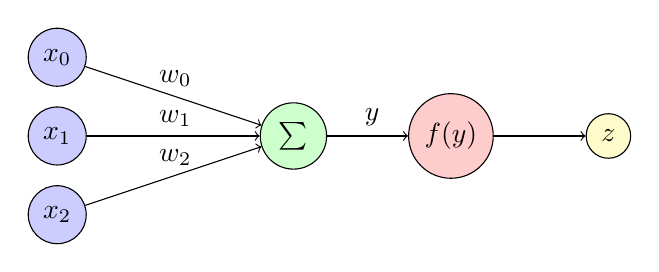
\begin{tikzpicture}

  % Input nodes
  \node[circle, draw, fill=blue!20] (x1) at (0,1) {$x_1$};
  \node[circle, draw, fill=blue!20] (x2) at (0,0) {$x_2$};

  % Weights
  \node[above] at (1.5,1) {$w_1$};
  \node[above] at (1.5,0.5) {$w_2$};

  % Sum node
  \node[circle, draw, fill=green!20] (sum) at (3,1) {$\sum$};
  \node[above] at (4,1) {$y$};

  % Activation node
  \node[circle, draw, fill=red!20] (activation) at (5,1) {$f(y)$};

  % Output node
  \node[circle, draw, fill=yellow!20] (output) at (7,1) {$z$};

  % Bias
  \node[circle, draw, fill=blue!20] (bias) at (0,2) {$x_0$};
  \node[above] at (1.5, 1.5) {$w_0$};

  % Connections
  \draw[->] (x1) -- (sum);
  \draw[->] (x2) -- (sum);
  \draw[->] (bias) -- (sum);
  \draw[->] (sum) -- (activation);
  \draw[->] (activation) -- (output);

\end{tikzpicture}
    \caption{Perceptron yang menerima tiga input dan mengeluarkan satu output}
    \label{fig: Perceptron}
\end{figure}

Gambar \ref{fig: Perceptron} menunjukan perceptron dengan tiga buah masukan yaitu $x_0$, $x_1$, dan $x_2$. 
bobot-bobot dituliskan dengan simbol $w_0$, $w_1$, dan $w_2$. 
Kemudian $y$ adalah kombinasi linier antara masukan dan bobotnya seperti pada Persamaan \ref{eq:wx+b}. 
Setelah melalui kombinasi linier keluaran diolah terlebih dahulu oleh fungsi $f(y)$. 
fungsi ini berfungsi untuk menentukan seberapa aktif neuron tersebut. 
fungsi ini disebut juga sebagai fungsi aktivasi pada jaringan syaraf tiruan modern. 
Terdapat berbagai macam fungsi aktivasi. Namun, pada awal perkembangan JST fungsi yang umum dipakai adalah fungsi yang menggunakan \textit{threshold} seperti \textit{step function}.

\begin{figure}[H]
    \centering
    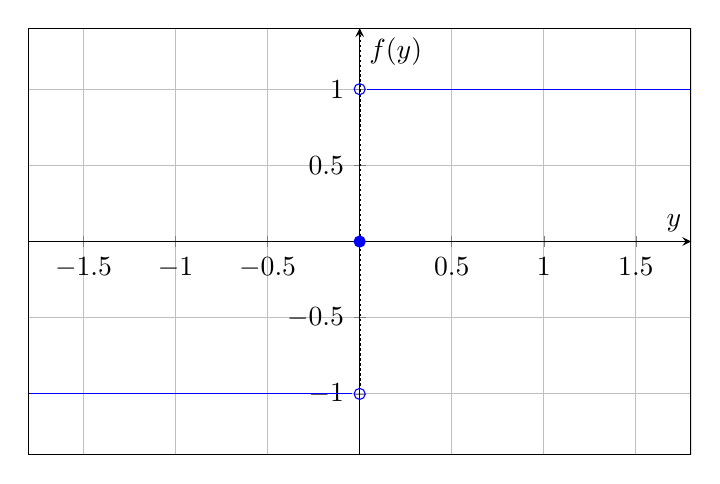
\begin{tikzpicture}
        \begin{axis}[
            xlabel=$y$,
            ylabel=$f(y)$,
            xmin=-1.8, xmax=1.8,
            ymin=-1.4, ymax=1.4,
            width=10cm,
            height=7cm,
            domain=-4:4,
            grid=both,
            samples=100,
            legend pos=south west,
            axis lines=middle, % Add this line to get the axes in the middle
        ]

        % Adding points
        \addplot[mark=*, color=blue, mark size = 2] coordinates {(0,0)};
        \addplot[mark=o, color=blue, mark size = 2] coordinates {(0,1)};
        \addplot[mark=o, color=blue, mark size = 2] coordinates {(0,-1)};

        % Adding line
        \draw[-, color=blue] (axis cs:0.04,1) -- (axis cs:2,1);
        \draw[-, color=blue] (axis cs:-2,-1) -- (axis cs:-0.04,-1);
        \draw[thick, densely dotted] (axis cs:0,96) -- (axis cs:0,-0.96);
        % Draw frame
        \draw[black, thick] (rel axis cs:0,0) rectangle (rel axis cs:1,1);
        \end{axis}
    \end{tikzpicture}
    \caption{Output fungsi aktivasi \textit{step function}}
    \label{fig:plot step_function}
\end{figure}

\textit{Step function} adalah salah satu fungsi aktivasi yang non linier dan tidak kontinu. Keluaran dari \textit{step function} dapat dilihat pada Gambar \ref{fig:plot step_function}. \textit{Step function} dapat ditulis seperti pada Persamaan \ref{eq: Step Function}.
\begin{equation}
    f(y) = 
    \begin{cases} 
    -1 & \text{jika } y < 0 \\
    1 & \text{jika } y \geq 0 
    \end{cases}
    \label{eq: Step Function}
\end{equation}
Pembelajaran \textit{perceptron algorithm} menggunakan \textit{perceptron criterion}. yaitu dengan menggunakan Persamaan \ref{eq: perceptron criterion} sebagai berikut:
\begin{equation}
    E_p(\textbf{w})=-\sum_{n \in M}^{}\textbf{w}^T \textbf{x}_n y_n
    \label{eq: perceptron criterion}
\end{equation}

Untuk menurunkannya, diasumsikan bahwa sebuah vektor bobot $\textbf{w}$ sedemikian sehingga setiap pola $\textbf{x}_n$ yang termasuk ke dalam kelas $C_1$ menghasilkan nilai
\begin{equation}
\textbf{w}^T \textbf{x}_n > 0,
\end{equation}
sedangkan pola yang termasuk ke dalam kelas $C_2$ menghasilkan nilai
\begin{equation}
\textbf{w}^T \textbf{x}_n < 0.
\end{equation}

Dengan menggunakan target \textit{expected value} sebagai $y_n \in \{-1, +1\}$, maka pola $x_n$ yang diklasifikasikan dengan benar akan memenuhi persamaan berikut:
\begin{equation}
\textbf{w}^T \textbf{x}_n y_n > 0,
\end{equation}

Pada \textit{perceptron criterion}, sebuah pola yang diklasifikasikan dengan benar
dianggap tidak memberikan \textit{error}. Sebaliknya, untuk pola yang
salah diklasifikasikan, fungsi error berusaha meminimalkan besaran
\begin{equation}
- \textbf{w}^T \textbf{x}_n y_n .
\end{equation}

Dengan demikian, Persamaan \ref{eq: perceptron criterion} mendefinisikan fungsi \textit{error} \textit{perceptron} di mana $M$ menyatakan himpunan seluruh pola yang salah diklasifikasikan. Bobot diperbarui menggunakan metode \textit{stochastic gradient descent}.
Aturan pembaruan bobot pada iterasi ke-$t$ dituliskan sebagai berikut:
\begin{equation}
\mathbf{w}^{(t+1)} = \mathbf{w}^{(t)} + \eta \, \mathbf{x}_n y_n,
\end{equation}
dengan $\eta$ menyatakan \textit{learning rate}.

\subsection{\textit{Multilayer Perceptron}}

Multilayer Perceptron (MLP) merupakan salah satu arsitektur jaringan syaraf tiruan \textit{feedforward} yang paling banyak digunakan dalam praktik \textit{machine learning} dan \textit{artificial intelligence}. 
MLP tersusun atas satu \textit{input layer}, satu atau lebih \textit{hidden layer}, serta satu \textit{output layer}, di mana setiap neuron pada suatu lapisan terhubung penuh (\textit{fully connected}) dengan neuron pada lapisan berikutnya \cite{Kelleher2019-cj}\cite{geron2019handson}\cite{publishing-2020}. 
Arsitektur ini banyak digunakan untuk tugas klasifikasi dan regresi karena kemampuannya dalam memodelkan hubungan non-linear antara data masukan dan keluaran.

Berbeda dengan perceptron tunggal yang hanya mampu menangani permasalahan yang bersifat \textit{linearly separable}, MLP menggunakan fungsi aktivasi non-linear pada \textit{hidden layer} sehingga mampu merepresentasikan pemetaan yang jauh lebih kompleks \cite{Bonaccorso2020-ec}\cite{knowings-2024}. 
Istilah \textit{multilayer perceptron} sendiri sebenarnya dianggap kurang tepat, karena unit pemrosesan yang digunakan bukan lagi perceptron klasik dengan fungsi aktivasi diskrit, melainkan neuron dengan fungsi aktivasi kontinu seperti \textit{sigmoid}, \textit{hyperbolic tangent}, atau \textit{ReLU} \cite{bishop_2006}. 
Jika seluruh lapisan dalam suatu jaringan hanya menggunakan transformasi linear, maka jaringan tersebut secara matematis dapat direduksi menjadi satu transformasi linear tunggal, sehingga keberadaan \textit{hidden layer} tidak memberikan keuntungan representasional \cite{bishop_2006}\cite{james-2022}.

Perkembangan MLP menjadi signifikan setelah diperkenalkannya algoritma \textit{backpropagation} oleh Rumelhart, Hinton, dan Williams pada tahun 1986 \cite{rumelhart-1986}. 
Algoritma ini memungkinkan perhitungan gradien \textit{error} terhadap setiap bobot jaringan secara efisien melalui dua tahap utama, yaitu propagasi maju (\textit{forward propagation}) dan propagasi balik (\textit{backpropagation}). 
Dengan mekanisme ini, kontribusi masing-masing bobot terhadap \textit{error} keluaran dapat ditentukan, sehingga bobot pada \textit{hidden layer} dapat diperbarui secara sistematis menggunakan metode optimasi berbasis \textit{gradient descent} \cite{Kelleher2019-cj}\cite{Luger2008-xe}. 
Tanpa adanya \textit{backpropagation}, pelatihan jaringan dengan banyak \textit{hidden layer} menjadi sangat sulit dilakukan \cite{Artificial-Intelligence-A-Guide-to-Intelligent-Systems}.

Dari sudut pandang kemampuan representasi, MLP telah terbukti sebagai \textit{universal function approximator}. 
Jaringan dengan satu \textit{hidden layer} dan jumlah neuron yang memadai secara teoritis mampu mendekati fungsi kontinu apa pun pada domain terbatas \cite{Guang-Bin}. 
Namun, dalam praktik, penggunaan beberapa \textit{hidden layer} dengan ukuran yang lebih kecil sering kali lebih efisien dibandingkan satu \textit{hidden layer} berukuran besar, baik dari segi jumlah parameter maupun kemudahan proses pelatihan \cite{james-2022}. 
Struktur bertingkat ini memungkinkan jaringan mengekstraksi \textit{feature} secara hierarkis, di mana lapisan awal mempelajari representasi sederhana, sedangkan lapisan yang lebih dalam mempelajari representasi yang lebih abstrak \cite{nelson-2023}.

MLP digunakan secara luas dalam berbagai aplikasi, khususnya pada tugas klasifikasi dan regresi. 
Pada tugas klasifikasi, \textit{output layer} umumnya menggunakan fungsi aktivasi seperti \textit{sigmoid} atau \textit{softmax}, sedangkan pada regresi sering digunakan neuron keluaran tanpa fungsi aktivasi untuk menghasilkan nilai kontinu \cite{publishing-2020}\cite{geron2019handson}. 
Fungsi kerugian yang umum digunakan dalam pelatihan MLP antara lain \textit{mean squared error} (MSE) dan \textit{cross-entropy} \cite{publishing-2020}. 
Meskipun memiliki kemampuan representasi yang tinggi, proses pelatihan MLP tetap menghadapi tantangan berupa konvergensi ke \textit{local minima} serta waktu komputasi yang relatif besar, terutama pada jaringan dengan banyak lapisan dan jumlah parameter yang besar \cite{bishop_2006}\cite{Artificial-Intelligence-A-Guide-to-Intelligent-Systems}.

\subsection{Proses Pelatihan}

Proses pelatihan pada Multilayer Perceptron (MLP) bertujuan untuk memperoleh nilai bobot yang optimal sehingga jaringan mampu menghasilkan keluaran yang mendekati nilai target. 
Proses ini dilakukan secara iteratif melalui beberapa tahap utama, yaitu forward propagation, perhitungan loss function, backpropagation, dan pembaruan bobot menggunakan metode optimasi tertentu.

\subsubsection{\textit{forward propagation}}
Forward propagation merupakan tahap awal dalam proses pelatihan MLP, di mana data masukan dipropagasikan dari \textit{input layer} menuju \textit{output layer}. 
Pada setiap neuron, sinyal masukan akan dikombinasikan secara linier dengan bobot yang bersesuaian dan ditambahkan dengan bias. 
Kombinasi linier tersebut kemudian dilewatkan ke fungsi aktivasi untuk menghasilkan keluaran neuron.

Secara umum, keluaran suatu neuron pada \textit{layer} ke-\( l \) dapat dituliskan sebagai :

\begin{equation}
    \mathbf{y}^{(l)}=f(\sum_{i}^{} \textbf{w}_{i}^{(l)} \textbf{x}_{i}^{(l-1)} + w_{0}^{(l)})
    \label{eq: forward propagation}
\end{equation}

di mana $\textbf{w}_{i}^{(l)}$ menyatakan vektor bobot, \( \textbf{x}_{i}^{(l)} \) menyatakan masukan \textit{neuron}, \( w_{0}^{(l)} \) adalah bias, dan \( f \) merupakan fungsi aktivasi. 
Proses ini dilakukan secara berurutan hingga diperoleh keluaran pada \textit{output layer} sebagai \textit{predicted value} dari jaringan.

\subsubsection{\textit{Loss Function}}

\textit{Loss function} adalah parameter yang digunakan untuk mengukur seberapa baik atau buruk kinerja suatu model dalam memprediksi nilai yang benar dari data yang 
diberikan. \textit{loss function} merupakan komponen penting dalam proses pelatihan model. Dengan menurunkan nilai \textit{loss function} model akan menjadi lebih baik 
\cite{GoodBengCour16}. Tujuan utama dari \textit{loss function} adalah untuk memberikan umpan balik kepada model terkait seberapa baik model tersebut memperkirakan 
nilai yang benar dari data yang diamati. Dengan kata lain, \textit{loss function} memberi tahu model seberapa jauh atau dekat prediksi model dengan nilai yang seharusnya.

\paragraph{\textit{Mean Square Error}}
\textit{Mean Squared Error} (MSE) merupakan fungsi loss yang paling umum digunakan pada permasalahan regresi. 
MSE mengukur rata-rata dari kuadrat selisih antara \textit{expected value} dan \textit{predicted value}.

\begin{equation}
    \text{MSE} = \frac{1}{N} \sum_{n=1}^{N} (y_n - \hat{y}_n)^2
    \label{eq:MSE}
\end{equation}

Dimana \(N\) adalah jumlah sampel data, \(y_n\) adalah \textit{expected value} dari sampel ke-n, \(\hat{y}_n\) adalah \textit{predicted value} oleh model untuk sampel ke-n. 
MSE memberikan penalti kuadrat terhadap \textit{error}, sehingga \textit{error} yang besar berdampak lebih signifikan terhadap nilai loss. 
Sifat ini membuat MSE sangat sensitif terhadap \textit{outlier}, tetapi juga mendorong model untuk menghasilkan prediksi yang sangat mendekati nilai target.
Selain itu, MSE memiliki turunan yang kontinu dan mudah dihitung, sehingga mempermudah optimasi menggunakan \textit{gradient descent}.

\paragraph{Fungsi Loss Lain}
Selain MSE, terdapat beberapa fungsi loss lain yang umum digunakan dalam berbagai konteks:

\begin{enumerate}
    \item Binary Cross-Entropy (BCE) digunakan untuk klasifikasi biner, mengukur perbedaan antara probabilitas prediksi dan label sebenarnya.

    \item Categorical Cross-Entropy (CCE) digunakan untuk klasifikasi multi-kelas.

    \item Huber Loss kombinasi MSE dan MAE, memiliki karakteristik lebih tahan terhadap outlier.

    \item Kullback–Leibler Divergence (KL Div) mengukur perbedaan dua distribusi probabilitas.
\end{enumerate}

Namun, karena penelitian ini berfokus pada data numerik dan pengaruh arsitektur jaringan terhadap akurasi, maka MSE dipilih sebagai fungsi loss utama.

\subsubsection{\textit{Backpropagation}}

\textit{Backpropagation} adalah algoritma yang digunakan untuk melatih jaringan saraf tiruan, khususnya pada model \textit{deep learning}. 
Algoritma ini memungkinkan jaringan untuk mengoptimalkan nilai bobot dan biasnya sehingga dapat meminimalkan nilai \textit{loss function} \cite{bishop_2006}. 
Istilah \textit{backpropagation} berasal dari \textit{backward propagation of errors}. 
Algoritma ini bekerja dengan menyebarkan \textit{error} dari \textit{output layer} ke lapisan-lapisan sebelumnya.

Proses \textit{backpropagation} terdiri dari dua tahap, yaitu \textit{forward pass} dan \textit{backward pass}. 
Pada tahap \textit{forward pass}, \textit{input} data dipropagasikan dari \textit{input layer} hingga \textit{output layer} untuk menghasilkan \textit{predicted value}. 
Kemudian, \textit{error} antara \textit{predicted value} (\( \hat{y} \)) dan \textit{expected value} (\( y \)) dihitung dengan \textit{loss function}.

Pada tahap backward pass, gradien \textit{loss function} terhadap keluaran jaringan dihitung, kemudian dipropagasikan kembali ke seluruh lapisan menggunakan aturan rantai (\textit{chain rule}). 
Nilai gradien ini menunjukkan seberapa besar kontribusi masing-masing bobot terhadap \textit{error} yang terjadi. 
Berdasarkan informasi tersebut, bobot dan bias diperbarui menggunakan metode optimisasi, seperti \textit{gradient descent}, agar \textit{error} pada iterasi berikutnya dapat dikurangi. 
Persamaan pembaruan bobot secara umum dapat dituliskan sebagai berikut:
\[
\textbf{w}^{(t+1)} = \textbf{w}^{(t)} - \eta \frac{\partial L}{\partial \textbf{w}}
\]
di mana \( \textbf{w} \) adalah vektor bobot, \( \eta \) adalah learning rate, dan \( \frac{\partial L}{\partial \textbf{w}} \) adalah gradien dari \textit{loss function} terhadap bobot tersebut. 
Langkah-langkah ini diulangi untuk setiap \textit{batch} data selama beberapa epoch sampai memenuhi kriteria tertentu. 
riteria tersebut dapat berupa \textit{loss function} konvergen ke nilai minimum, \textit{predicted value} sudah serupa dengan \textit{expected value}, 
iterasi mencapai jumlah yang ditentukan, atau dengan membandingkan bobot sebelum dan sesudah pembaruannya dengan \textit{relative error}.

\subsubsection{Gradient Descent}

Gradient descent adalah algoritma optimasi yang digunakan untuk meminimalkan \textit{loss function} dalam berbagai model pembelajaran mesin dan jaringan saraf tiruan. 
Inti dari algoritma ini adalah memperbarui parameter model secara iteratif untuk mengurangi nilai \textit{loss function} \cite{bishop_2006}. Proses ini dilakukan dengan 
mengikuti arah gradien dari \textit{loss function}.
\begin{equation}
    \theta_{t+1} = \theta_t - \eta \nabla_\theta J(\theta_t)
    \label{eq:pembaharuan bobot}
\end{equation}
Dimana $(\theta_t)$ adalah parameter pada iterasi ke-\(t\). \(\eta\) adalah laju pembelajaran (\textit{learning rate}). \(\nabla_\theta J(\theta_t)\) adalah gradien 
dari \textit{loss function} \(J\) terhadap parameter \(\theta\) pada iterasi ke-\(t\). Cara kerja \textit{gradient descent} dimulai dengan inisialisasi parameter 
model $(\theta)$ secara acak atau dengan nilai tertentu. Setelah itu, \textit{loss function} $J(\theta)$ dievaluasi berdasarkan parameter saat ini dan data pelatihan. 
Langkah selanjutnya adalah menghitung gradien dari \textit{loss function} terhadap parameter. Gradien adalah vektor yang menunjukkan arah dan laju perubahan dari 
\textit{loss function}, yang secara matematis dinyatakan sebagai $\nabla_\theta J(\theta)$. Parameter kemudian diperbarui dengan bergerak ke arah gradien negatif 
untuk mengurangi nilai \textit{loss function}. Pembaruan parameter dilakukan dengan menggunakan persamaan \ref{eq:pembaharuan bobot}, dimana $\eta$ adalah learning rate 
yang menentukan ukuran langkah yang diambil menuju minimum \textit{loss function}. Langkah-langkah ini diulangi sampai \textit{loss function} konvergen ke nilai minimum 
atau perubahan dalam \textit{loss function} menjadi sangat kecil.

\paragraph{Varian Gradient Descent}
Gradient descent adalah algoritma inti dalam optimasi model pembelajaran mesin. Dengan memilih varian yang sesuai dan menggunakan teknik optimasi, model dapat dilatih dengan lebih efisien dan efektif, mencapai konvergensi yang lebih cepat dan hasil yang lebih baik.

\begin{enumerate}
    \item Batch Gradient Descent: Menggunakan seluruh dataset untuk menghitung gradien dan memperbarui parameter \cite{GoodBengCour16}. Kelebihannya adalah konvergen menuju minimum global dengan lebih stabil, namun memerlukan komputasi yang besar jika dataset sangat besar.
    
    \item Stochastic Gradient Descent (SGD): Menggunakan satu sampel data untuk menghitung gradien dan memperbarui parameter \cite{GoodBengCour16}. Kelebihannya adalah lebih cepat dan lebih efisien untuk dataset besar, namun gradien yang dihitung akan memiliki \textit{noise} sehingga jalur konvergensi bisa lebih berliku-liku.

    \item Mini-Batch Gradient Descent: Kombinasi antara batch gradient descent dan SGD. Menggunakan batch kecil (mini-batch) dari dataset untuk menghitung gradien dan memperbarui parameter \cite{GoodBengCour16}. Pendekatan ini menggabungkan kecepatan dan efisiensi dari SGD dengan kestabilan batch gradient descent.
\end{enumerate}

Untuk meningkatkan stabilitas dan kecepatan konvergensi, SGD dapat dikombinasikan dengan metode momentum. Metode momentum memperhitungkan arah pembaruan bobot sebelumnya sehingga dapat mengurangi osilasi dan membantu jaringan keluar dari local minima. 
Selain itu, terdapat metode optimasi lain seperti Adam yang mengadaptasi laju pembelajaran secara otomatis untuk setiap bobot, meskipun tidak selalu digunakan pada setiap penelitian.

Karena dataset yang digunakan pada penelitian ini relatif kecil dan model bersifat linier, maka algoritma Batch Gradient Descent dipilih untuk menjamin konvergensi 
yang stabil menuju solusi optimal. Penggunaan seluruh dataset pada setiap pembaruan bobot memastikan bahwa arah gradien yang dihitung benar-benar merepresentasikan 
keseluruhan distribusi data.



\subsection{Normalisasi}

Normalisasi adalah proses mengubah skala data agar setiap \textit{feature} memiliki rentang nilai atau distribusi tertentu yang diinginkan. 
Nilai \textit{feature} yang bervariasi secara signifikan dapat memengaruhi stabilitas proses pelatihan jaringan saraf tiruan. 
Pada algoritma \textit{gradient descent}, pembaruan bobot dilakukan berdasarkan \textit{gradien} dari fungsi \textit{loss}. 
Jika skala antar \textit{feature} berbeda jauh, \textit{gradien} yang dihasilkan juga menjadi tidak seimbang. 
\textit{feature} dengan nilai besar cenderung menghasilkan pembaruan bobot yang terlalu besar, sedangkan \textit{feature} dengan nilai kecil menghasilkan pembaruan yang lambat. 
Akibatnya, proses konvergensi dapat menjadi tidak stabil atau bahkan gagal \cite{Langr2019-xk}.

Sebagai ilustrasi diberikan data seperti pada Tabel \ref{tab:hargarumah} yang menunjukan harga rumah di Jakarta.

\begin{table}[H]
    \centering
    \begin{tabular}{||p{5em}|p{5em}|p{5em}|p{5em}|p{6em}||}
    \hline
       Luas Tanah (m²) & Jumlah Kamar Tidur & Usia Rumah (tahun) & Jarak ke Pusat Kota (km) & Harga Rumah (IDR)\\ [0.5ex]
        \hline\hline
       300 & 3 & 10 & 15 & 1,500,000,000\\ \hline
       500 & 4 & 5 & 10 & 2,000,000,000\\ \hline
       450 & 3 & 20 & 20 & 1,750,000,000\\ \hline
       600 & 5 & 8 & 5 &2,500,000,000\\ \hline
    \end{tabular}
    \caption{Data \textit{dummy} harga rumah di Jakarta}
    \label{tab:hargarumah}
\end{table}

Jika \textit{raw} data ini langsung digunakan ke algoritma pembelajaran seperti regresi linear atau jaringan syaraf tiruan, \textit{feature} "luas tanah" akan mendominasi proses 
pelatihan karena memiliki skala yang jauh lebih besar dibandingkan "Jumlah Kamar Tidur" hal ini akan menimbulkan bias bahwa "luas tanah" lebih penting dari "Jumlah Kamar Tidur". 
Untuk mengatasi masalah ini, dapat dilakukan normalisasi pada setiap \textit{feature} sehingga semua \textit{feature} memiliki skala yang serupa. 
Salah satu metode normalisasi yang umum adalah Min-Max Scaling, yang mengubah skala setiap \textit{feature} ke dalam rentang 0 hingga 1. 
Persamaan \textit{Min-Max Scaling} (\ref{eq:minmax})dituliskan sebagai berikut:

\begin{equation}
    x_{norm} = \frac{x-x_{min}}{x_{max}-x_{min}}
    \label{eq:minmax}
\end{equation}

Selain \textit{Min-max scaling}, terdapat metode normalisasi lain  yaitu \textit{Z-score standardization}. \textit{Z-score standardization} adalah metode normalisasi 
data yang mengubah data sehingga memiliki nilai rata-rata 0 dan standar deviasi 1 \cite{Langr2019-xk}. Persamaan \textit{Z-score standardization} (\ref{eq:Zscore}):

\begin{equation}
    Z=\frac{X-\mu}{\sigma}
    \label{eq:Zscore}
\end{equation}

Dengan normalisasi, setiap \textit{feature} berkontribusi secara proporsional terhadap proses pembelajaran jaringan, sehingga mempercepat konvergensi, menstabilkan pelatihan, dan 
meningkatkan akurasi prediksi model.

\subsection{\textit{Relative error}}

Relative error adalah ukuran ketidakakuratan dalam pengukuran atau estimasi yang dinyatakan sebagai perbandingan antara \textit{absolute error} dan \textit{true value}. Persamaan dapat ditulis sebagai berikut :
\begin{equation}
    \text{Relative Error} = \frac{\text{Absolute Error}}{\text{True Value}}
\end{equation}
Dimana \textit{Absolute Error} pada konteks ini adalah selisih antara \textit{True Value} dan \textit{Measured Value}. Dalam pelatihan jaringan syaraf tiruan, \textit{relative error} sering 
digunakan sebagai kriteria penghentian untuk menentukan kapan pelatihan harus dihentikan. Penggunaan \textit{relative error} sebagai parameter penghentian memiliki 
beberapa manfaat penting. Pertama, ini memungkinkan pelatihan dihentikan ketika \textit{relative error} mencapai nilai yang cukup kecil, menunjukkan bahwa model 
telah mencapai tingkat akurasi yang diinginkan. Kedua, ini membantu mencegah \textit{overfitting}, dimana model menjadi terlalu terlatih pada data pelatihan dan tidak 
dapat digeneralisasi dengan baik pada data baru. Ketiga, penggunaan \textit{relative error} sebagai kriteria penghentian menghemat waktu dan sumber daya komputasi, 
karena pelatihan lebih lanjut mungkin tidak memberikan peningkatan signifikan dalam performa model. Terakhir, \textit{relative error} memberikan penilaian kinerja yang 
bersifat relatif terhadap skala nilai yang diukur, sehingga memudahkan evaluasi dan perbandingan kinerja model pada berbagai dataset atau aplikasi yang berbeda. Dengan 
demikian, \textit{relative error} sebagai parameter pemberhenti memastikan bahwa pelatihan JST dilakukan secara efisien dan menghasilkan model yang memiliki kinerja baik pada data.




